% Options for packages loaded elsewhere
\PassOptionsToPackage{unicode}{hyperref}
\PassOptionsToPackage{hyphens}{url}
%
\documentclass[
]{book}
\usepackage{amsmath,amssymb}
\usepackage{iftex}
\ifPDFTeX
  \usepackage[T1]{fontenc}
  \usepackage[utf8]{inputenc}
  \usepackage{textcomp} % provide euro and other symbols
\else % if luatex or xetex
  \usepackage{unicode-math} % this also loads fontspec
  \defaultfontfeatures{Scale=MatchLowercase}
  \defaultfontfeatures[\rmfamily]{Ligatures=TeX,Scale=1}
\fi
\usepackage{lmodern}
\ifPDFTeX\else
  % xetex/luatex font selection
\fi
% Use upquote if available, for straight quotes in verbatim environments
\IfFileExists{upquote.sty}{\usepackage{upquote}}{}
\IfFileExists{microtype.sty}{% use microtype if available
  \usepackage[]{microtype}
  \UseMicrotypeSet[protrusion]{basicmath} % disable protrusion for tt fonts
}{}
\makeatletter
\@ifundefined{KOMAClassName}{% if non-KOMA class
  \IfFileExists{parskip.sty}{%
    \usepackage{parskip}
  }{% else
    \setlength{\parindent}{0pt}
    \setlength{\parskip}{6pt plus 2pt minus 1pt}}
}{% if KOMA class
  \KOMAoptions{parskip=half}}
\makeatother
\usepackage{xcolor}
\usepackage{color}
\usepackage{fancyvrb}
\newcommand{\VerbBar}{|}
\newcommand{\VERB}{\Verb[commandchars=\\\{\}]}
\DefineVerbatimEnvironment{Highlighting}{Verbatim}{commandchars=\\\{\}}
% Add ',fontsize=\small' for more characters per line
\usepackage{framed}
\definecolor{shadecolor}{RGB}{248,248,248}
\newenvironment{Shaded}{\begin{snugshade}}{\end{snugshade}}
\newcommand{\AlertTok}[1]{\textcolor[rgb]{0.94,0.16,0.16}{#1}}
\newcommand{\AnnotationTok}[1]{\textcolor[rgb]{0.56,0.35,0.01}{\textbf{\textit{#1}}}}
\newcommand{\AttributeTok}[1]{\textcolor[rgb]{0.13,0.29,0.53}{#1}}
\newcommand{\BaseNTok}[1]{\textcolor[rgb]{0.00,0.00,0.81}{#1}}
\newcommand{\BuiltInTok}[1]{#1}
\newcommand{\CharTok}[1]{\textcolor[rgb]{0.31,0.60,0.02}{#1}}
\newcommand{\CommentTok}[1]{\textcolor[rgb]{0.56,0.35,0.01}{\textit{#1}}}
\newcommand{\CommentVarTok}[1]{\textcolor[rgb]{0.56,0.35,0.01}{\textbf{\textit{#1}}}}
\newcommand{\ConstantTok}[1]{\textcolor[rgb]{0.56,0.35,0.01}{#1}}
\newcommand{\ControlFlowTok}[1]{\textcolor[rgb]{0.13,0.29,0.53}{\textbf{#1}}}
\newcommand{\DataTypeTok}[1]{\textcolor[rgb]{0.13,0.29,0.53}{#1}}
\newcommand{\DecValTok}[1]{\textcolor[rgb]{0.00,0.00,0.81}{#1}}
\newcommand{\DocumentationTok}[1]{\textcolor[rgb]{0.56,0.35,0.01}{\textbf{\textit{#1}}}}
\newcommand{\ErrorTok}[1]{\textcolor[rgb]{0.64,0.00,0.00}{\textbf{#1}}}
\newcommand{\ExtensionTok}[1]{#1}
\newcommand{\FloatTok}[1]{\textcolor[rgb]{0.00,0.00,0.81}{#1}}
\newcommand{\FunctionTok}[1]{\textcolor[rgb]{0.13,0.29,0.53}{\textbf{#1}}}
\newcommand{\ImportTok}[1]{#1}
\newcommand{\InformationTok}[1]{\textcolor[rgb]{0.56,0.35,0.01}{\textbf{\textit{#1}}}}
\newcommand{\KeywordTok}[1]{\textcolor[rgb]{0.13,0.29,0.53}{\textbf{#1}}}
\newcommand{\NormalTok}[1]{#1}
\newcommand{\OperatorTok}[1]{\textcolor[rgb]{0.81,0.36,0.00}{\textbf{#1}}}
\newcommand{\OtherTok}[1]{\textcolor[rgb]{0.56,0.35,0.01}{#1}}
\newcommand{\PreprocessorTok}[1]{\textcolor[rgb]{0.56,0.35,0.01}{\textit{#1}}}
\newcommand{\RegionMarkerTok}[1]{#1}
\newcommand{\SpecialCharTok}[1]{\textcolor[rgb]{0.81,0.36,0.00}{\textbf{#1}}}
\newcommand{\SpecialStringTok}[1]{\textcolor[rgb]{0.31,0.60,0.02}{#1}}
\newcommand{\StringTok}[1]{\textcolor[rgb]{0.31,0.60,0.02}{#1}}
\newcommand{\VariableTok}[1]{\textcolor[rgb]{0.00,0.00,0.00}{#1}}
\newcommand{\VerbatimStringTok}[1]{\textcolor[rgb]{0.31,0.60,0.02}{#1}}
\newcommand{\WarningTok}[1]{\textcolor[rgb]{0.56,0.35,0.01}{\textbf{\textit{#1}}}}
\usepackage{longtable,booktabs,array}
\usepackage{calc} % for calculating minipage widths
% Correct order of tables after \paragraph or \subparagraph
\usepackage{etoolbox}
\makeatletter
\patchcmd\longtable{\par}{\if@noskipsec\mbox{}\fi\par}{}{}
\makeatother
% Allow footnotes in longtable head/foot
\IfFileExists{footnotehyper.sty}{\usepackage{footnotehyper}}{\usepackage{footnote}}
\makesavenoteenv{longtable}
\usepackage{graphicx}
\makeatletter
\def\maxwidth{\ifdim\Gin@nat@width>\linewidth\linewidth\else\Gin@nat@width\fi}
\def\maxheight{\ifdim\Gin@nat@height>\textheight\textheight\else\Gin@nat@height\fi}
\makeatother
% Scale images if necessary, so that they will not overflow the page
% margins by default, and it is still possible to overwrite the defaults
% using explicit options in \includegraphics[width, height, ...]{}
\setkeys{Gin}{width=\maxwidth,height=\maxheight,keepaspectratio}
% Set default figure placement to htbp
\makeatletter
\def\fps@figure{htbp}
\makeatother
\setlength{\emergencystretch}{3em} % prevent overfull lines
\providecommand{\tightlist}{%
  \setlength{\itemsep}{0pt}\setlength{\parskip}{0pt}}
\setcounter{secnumdepth}{5}
\usepackage{booktabs}
\ifLuaTeX
  \usepackage{selnolig}  % disable illegal ligatures
\fi
\usepackage[]{natbib}
\bibliographystyle{plainnat}
\usepackage{bookmark}
\IfFileExists{xurl.sty}{\usepackage{xurl}}{} % add URL line breaks if available
\urlstyle{same}
\hypersetup{
  pdftitle={Machine Learning in Genomics: Containerised tutorials demonstrating best practises, pitfalls, and reproducibility},
  pdfauthor={ Sach Nehal},
  hidelinks,
  pdfcreator={LaTeX via pandoc}}

\title{Machine Learning in Genomics: Containerised tutorials demonstrating best practises, pitfalls, and reproducibility}
\author{Sach Nehal}
\date{2024-07-10}

\begin{document}
\maketitle

{
\setcounter{tocdepth}{1}
\tableofcontents
}
\chapter*{About}\label{about}
\addcontentsline{toc}{chapter}{About}

Applied machine learning utilising vast amounts of data has aided in pattern identification, predictive analytics, and solving complex problems across a multitude of fields. Solving these complex problems within these fields, researchers would find differing answers to the following questions; \textbf{what machine learning techniques can we apply to the problem, how do we apply the techniques in the context of this field, and why do we need to apply them in this way?} In any case, applied machine learning requires an interdisciplinary understanding of computing techniques and the field in question.

The aim of this project is to provide you with \textbf{a set of reproducible, containerized tutorials that include all necessary data, code, and descriptions to replicate key results, along with demonstrations of common pitfalls, in the field of genomics}. It is designed for users with knowledge of machine learning but little or no background in biology as a process to learn about applying machine learning techniques in genomics.

\part{Introduction}\label{part-introduction}

\chapter{Epigenetic Data}\label{epigenetic-data}

\section{What is epigenetic data?}\label{what-is-epigenetic-data}

As you may already know, typically all of the cells in your body contain the same DNA. How, then, do we have different cell types in our body? Your DNA contains a script that is able to produce the proteins required for each specific cell in your body. Which proteins, and subsequently which cells are made, depends on gene expression and regulation, i.e.~``the way each cell deploys its genome.''\footnote{\citet{ralston2008}}

\textbf{\emph{Epigenetic data}} arises from ``the study of heritable and stable changes in gene expression that occur through alterations in the chromosome rather than in the DNA sequence.''\footnote{\citet{nora2023}}

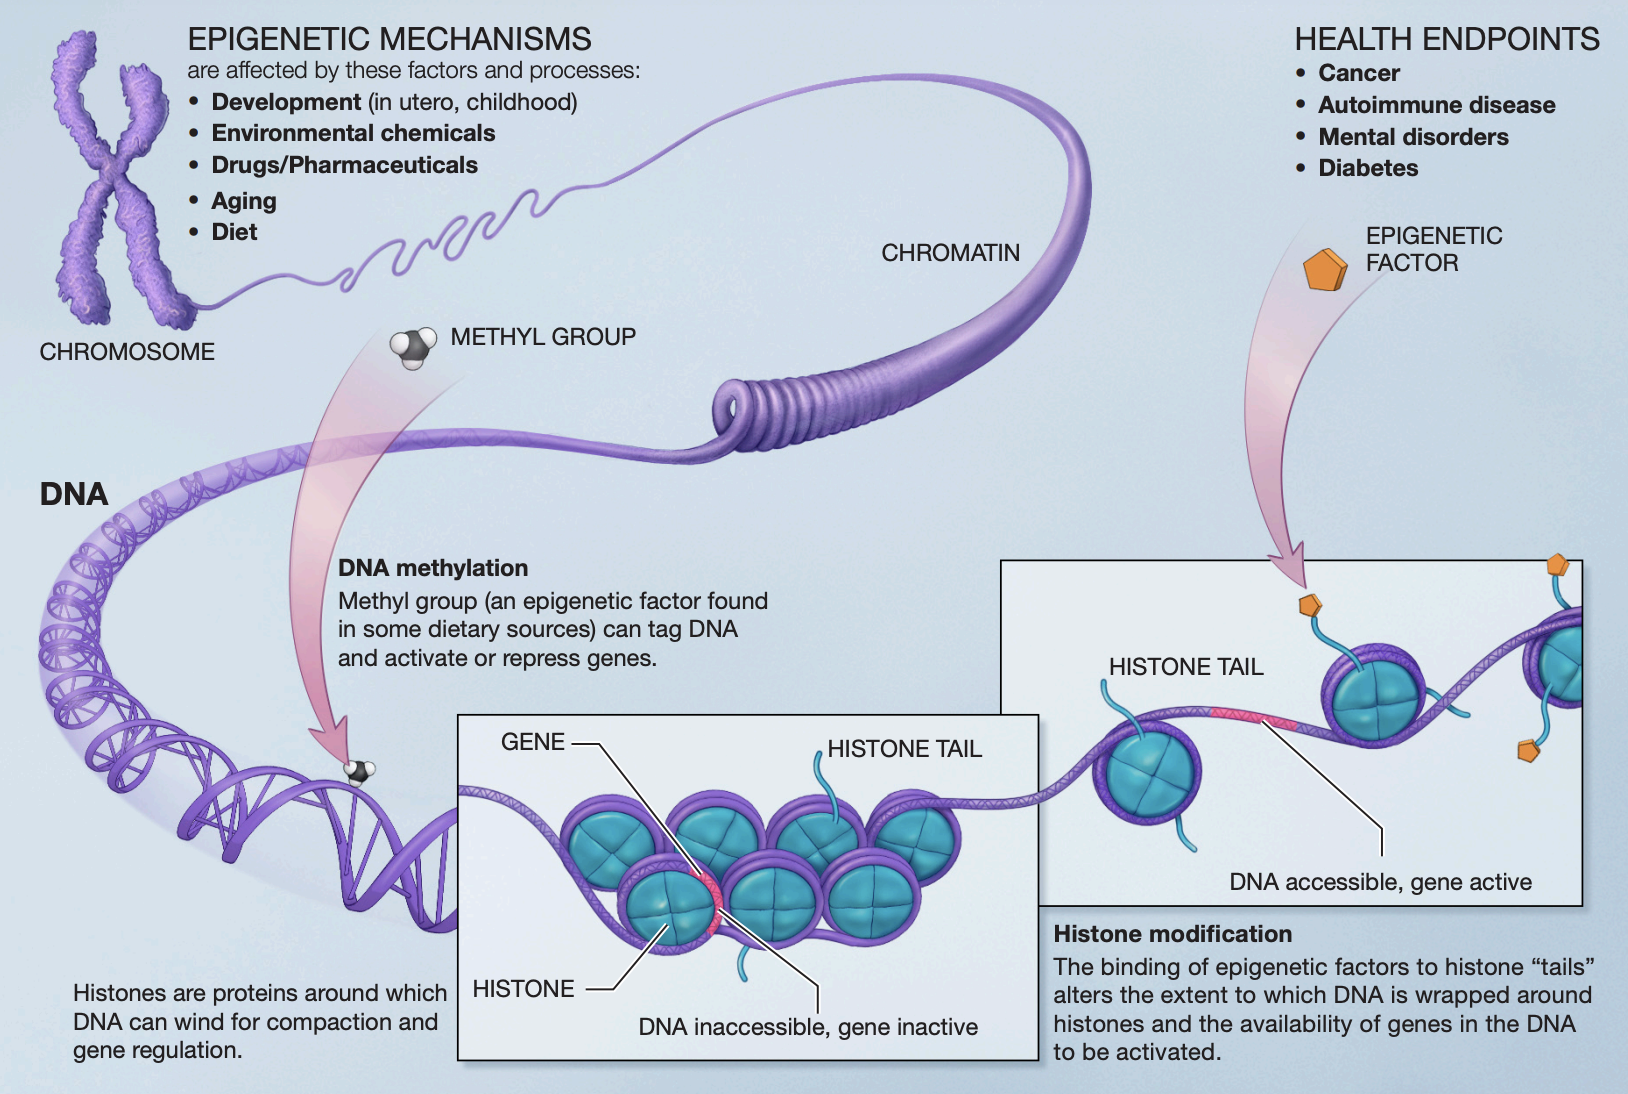
\includegraphics{images/Epigenetic_Mechanisms.png}

\href{https://commonfund.nih.gov/sites/default/files/epigeneticmechanisms.pdf}{commonfund.nih.gov}

The image above shows quite simply the basics of genetic structures. Several more complex processes are involved during cell replication such as DNA transcription and translation in order to make proteins. A key takeaway in coming closer to understanding gene expression is that \textbf{Chromatin} is a complex structure made up of DNA wound around histone proteins, with some segments of DNA being accessible/inaccessible to further processes. \textbf{Euchromatin} refers to the accessible state, while \textbf{Heterochromatin} refers to a chromatin state in which DNA cannot be transcribed (inaccessible).\footnote{\citet{shahid2023}} There are many different epigenetic modifications that affect chromatin accessibility.

Some common epigenetic modifications include:

\begin{enumerate}
\def\labelenumi{\arabic{enumi}.}
\tightlist
\item
  \textbf{DNA Methylation}: Addition of methyl groups to DNA, affecting gene expression regulation\footnote{\citet{nora2023}}.
\item
  \textbf{Histone Modifications}: Chemical changes to histone proteins that DNA wraps around, including acetylation, methylation, or phosphorylation. These changes influence chromatin structure and gene accessibility.\footnote{\citet{Kouzarides2007}}
\item
  \textbf{Chromatin Accessibility}: Regions of open chromatin that are accessible to transcription factors (special types of proteins that bind to DNA sequences and regulate gene expression) further dictate which regions of DNA can be expressed\footnote{\citet{melanie2021}}.
\end{enumerate}

In studying gene expression and epigenetic modifications, we can more closely understand biological mechanisms that regulate development, disease, and how cells respond to epigenetic factors.

\subsection{Common Epigenetic Techniques:}\label{common-epigenetic-techniques}

\begin{enumerate}
\def\labelenumi{\arabic{enumi}.}
\item
  \textbf{\emph{ATAC-Seq}} (Assay for Transposase-Accessible Chromatin with Sequencing):
  o\texttt{Measures\ chromatin\ accessibility\ to\ identify\ open\ regions\ of\ the\ genome\ where\ transcription\ factors\ can\ bind.}
  o\texttt{Output:\ Peaks\ indicating\ accessible\ chromatin\ regions.}
\item
  \textbf{\emph{ChIP-Seq}} (Chromatin Immunoprecipitation Sequencing):
  o\texttt{Used\ to\ identify\ DNA\ regions\ bound\ by\ specific\ proteins\ (e.g.,\ transcription\ factors,\ histones\ with\ specific\ modifications).}
  o\texttt{Output:\ Peaks\ indicating\ binding\ sites\ or\ modification\ locations.}
\end{enumerate}

\section{What does epigenetic data look like?}\label{what-does-epigenetic-data-look-like}

Epigenetic data can be represented in various forms, depending on the type of modification being studied and the methods used to gather the data. \textbf{ATAC-Seq} and \textbf{ChIP-Seq} are the common methods I will focus on, but there are others that may produce different forms of data, such as WGS (whole-genome sequencing) which produces nucleotide sequencing data, or Bisulfite conversion of DNA producing data on methylation levels across the genome.

\subsection{Representing epigenetic data}\label{representing-epigenetic-data}

\begin{enumerate}
\def\labelenumi{\arabic{enumi}.}
\tightlist
\item
  \textbf{\emph{Raw Sequence Reads:}}
  o\texttt{These\ are\ the\ basic\ output\ of\ sequencing\ experiments,\ such\ as\ those\ from\ ChIP-Seq\ or\ ATAC-Seq.}
  o\texttt{Reads\ are\ processed\ and\ aligned\ to\ a\ reference\ genome\ before\ undergoing\ peak\ calling.}
\item
  \textbf{\emph{Peak Calling:}}
  o\texttt{A\ method\ used\ to\ identify\ regions\ in\ the\ genome\ where\ there\ is\ significant\ enrichment\ of\ sequencing\ reads.\ This\ indicates\ the\ presence\ of\ DNA-protein\ interactions\ (e.g.,\ transcription\ factor\ binding\ sites)\ or\ accessible\ chromatin\ regions.}
  o\texttt{Peaks\ represent\ areas\ where\ epigenetic\ marks\ or\ chromatin\ accessibility\ are\ concentrated.}
\end{enumerate}

\textbf{\emph{Representing Peaks:}}
o \textbf{\emph{P-value or Fold-change:}}
P-value: Indicates the statistical significance of the peak, helping to distinguish true peaks from background noise.
Fold-change: Represents the difference in read density between treated and control samples, indicating the strength of the signal.
o \textbf{\emph{Types of Peaks:}}
Categorical Peaks: Simple yes/no indication of a peak's presence.
Continuous Peaks: More nuanced representation that includes the intensity or enrichment level of the peak, often visualized as a signal track.
Thresholded/Pseudoreplicated Peaks: Usually categorical, these peaks are of high confidence regions from multiple replicates (experiments) or pseudoreplicates (artificial data splits), to ensure reliability and reproducibility.

\textbf{\emph{Example Data Pipeline}}

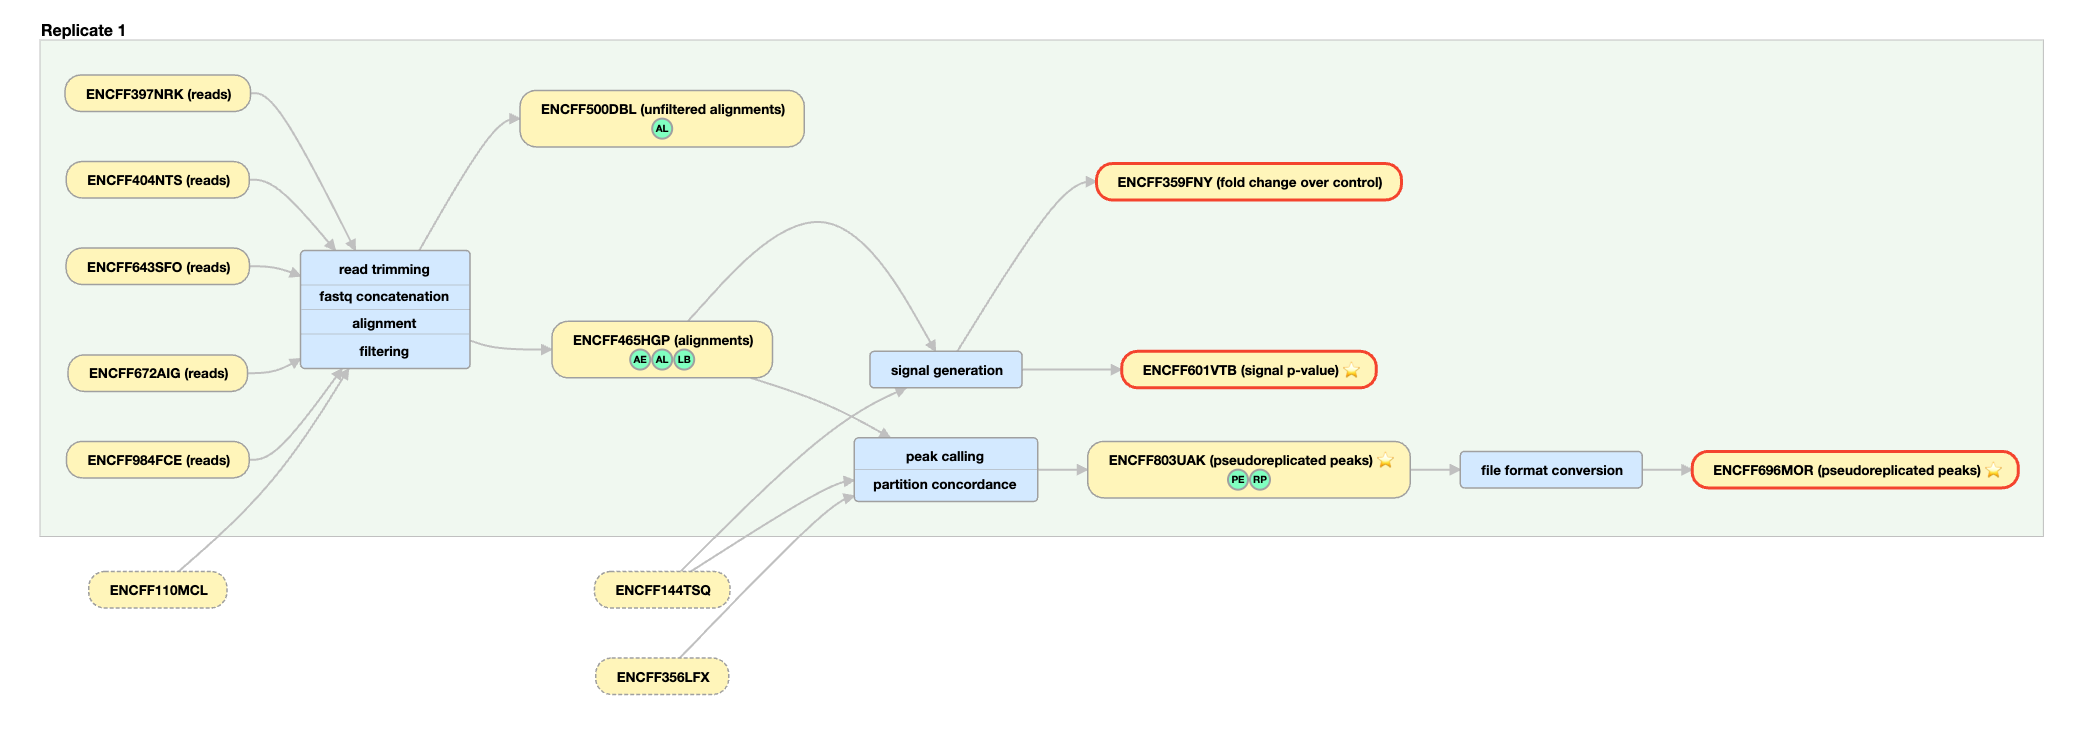
\includegraphics{images/chIP-Seq_pipeline.png}

\href{https://www.encodeproject.org/experiments/ENCSR817LUF/}{encodeproject.org}

This example data pipeline originates from a ChIP-seq experiment targeting the H3K36me3 histone modification in brain tissue. The aim of the experiement is to map the locations where the H3K36me3 histone modification is present along the genome. The yellow bubbles represent downloadable data sets of different types, while the blue boxes represent step types (e.g.~peak calling). In the left column are multiple data sets of raw sequence reads, which then undergo data quality steps before being aligned (first blue box) to the reference human genome GRCh38 (denoted by ENCFF110MCL below the reads). The next steps include Peak calling (categorical peaks) and signal generation (continuous peaks) to produce the data we normally use in our machine learning models. This data pipeline process aids in normalisation, noise reduction, and dimensionality reduction of the data.

\subsection{Example Data Representations:}\label{example-data-representations}

The following is an example of what this same chIP-Seq data targeting the H3K36me3 histone modification in brain tissue looks like using UCSC's Genome Browser. The pseudoreplicated peaks represent categorically, the significant locations along the genome where the H3K36me3 histone modification is present.

\href{https://genome.ucsc.edu/cgi-bin/hgTracks?db=hg38&lastVirtModeType=default&lastVirtModeExtraState=&virtModeType=default&virtMode=0&nonVirtPosition=&position=chr1\%3A11084744\%2D11095920&hgsid=2307713234_Kap236Tjt6ZGnnNrXMkIhq2Ajn27}{UCSC Genome Browser}

\href{https://www.encodeproject.org/experiments/ENCSR875FZN/}{encodeproject.org}

\subsection{Transformations to stop extreme p-values}\label{transformations-to-stop-extreme-p-values}

Arcsinh-transformation

\section{Sources of epigenetic data}\label{sources-of-epigenetic-data}

Blueprint
Roadmap
Encode (Main Focus)

\section{Handling bigWig files}\label{handling-bigwig-files}

\section{Data loaders and pre-processing}\label{data-loaders-and-pre-processing}

\section{Dealing with missing data (oversampling, undersampling, weighting)}\label{dealing-with-missing-data-oversampling-undersampling-weighting}

\#\#testpython code

\begin{Shaded}
\begin{Highlighting}[]
\ImportTok{import}\NormalTok{ numpy }\ImportTok{as}\NormalTok{ np}
\ImportTok{import}\NormalTok{ matplotlib.pyplot }\ImportTok{as}\NormalTok{ plt}

\NormalTok{x }\OperatorTok{=}\NormalTok{ np.linspace(}\DecValTok{0}\NormalTok{, }\DecValTok{10}\NormalTok{, }\DecValTok{100}\NormalTok{)}
\NormalTok{y }\OperatorTok{=}\NormalTok{ np.sin(x)}

\NormalTok{plt.plot(x, y)}
\NormalTok{plt.xlabel(}\StringTok{\textquotesingle{}x\textquotesingle{}}\NormalTok{)}
\NormalTok{plt.ylabel(}\StringTok{\textquotesingle{}y\textquotesingle{}}\NormalTok{)}
\NormalTok{plt.title(}\StringTok{\textquotesingle{}Sine Wave\textquotesingle{}}\NormalTok{)}
\NormalTok{plt.grid(}\VariableTok{True}\NormalTok{)}
\NormalTok{plt.savefig(}\StringTok{\textquotesingle{}images/sine\_wave.png\textquotesingle{}}\NormalTok{)}
\NormalTok{plt.show()}
\end{Highlighting}
\end{Shaded}

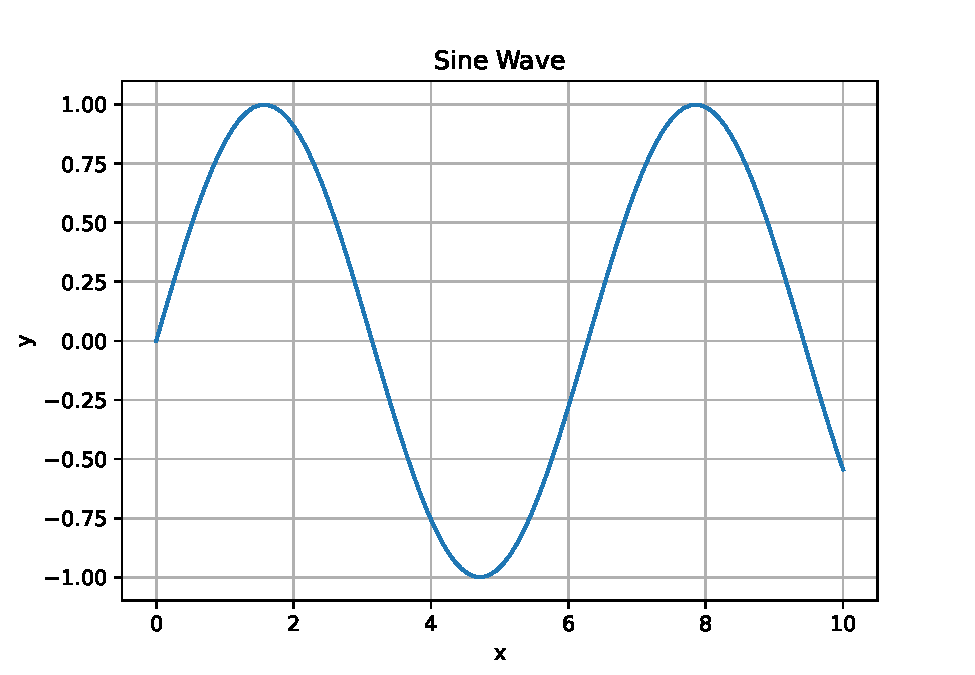
\includegraphics{_main_files/figure-latex/unnamed-chunk-2-1.pdf}

\part{Training models with DNA input}\label{part-training-models-with-dna-input}

\chapter{Loss functions, and peak metrics}\label{loss-functions-and-peak-metrics}

\chapter{Base pair averaging}\label{base-pair-averaging}

\chapter{Training tricks}\label{training-tricks}

\chapter{Choosing which genomic regions to train on}\label{choosing-which-genomic-regions-to-train-on}

\chapter{Effect of differences in sequencing depths}\label{effect-of-differences-in-sequencing-depths}

\chapter{Reproducibility of machine learning models}\label{reproducibility-of-machine-learning-models}

\section{Seeding}\label{seeding}

\section{Dashboarding}\label{dashboarding}

\chapter{Testing}\label{testing}

\part{Software libraries for model building}\label{part-software-libraries-for-model-building}

\chapter{gReLU}\label{grelu}

\chapter{Kipoi}\label{kipoi}

\chapter{Weights and Biases}\label{weights-and-biases}

\part{ML pitfalls in genomics}\label{part-ml-pitfalls-in-genomics}

\chapter{Pitfalls overview}\label{pitfalls-overview}

\section{Distributional differences}\label{distributional-differences}

\section{Dependent examples}\label{dependent-examples}

\section{Confounding}\label{confounding}

\section{Leaky pre-processing}\label{leaky-pre-processing}

\section{Unbalanced classes}\label{unbalanced-classes}

\section{Balancing the proportion of peaks / no-peaks in validation sets}\label{balancing-the-proportion-of-peaks-no-peaks-in-validation-sets}

\part{Model interpretability}\label{part-model-interpretability}

\chapter{Creating and visualising a simple model}\label{creating-and-visualising-a-simple-model}

\chapter{TF mo-Disco}\label{tf-mo-disco}

\part{Using existing models}\label{part-using-existing-models}

\chapter{Using the gReLU model zoo}\label{using-the-grelu-model-zoo}

\chapter{Fine tuning of Enformer}\label{fine-tuning-of-enformer}

\part{Predicting in novel cell types}\label{part-predicting-in-novel-cell-types}

\chapter{Incorporating ATAC-seq info}\label{incorporating-atac-seq-info}

\chapter{Use of cell type averages}\label{use-of-cell-type-averages}

\part{More complex models}\label{part-more-complex-models}

\chapter{Training multi-headed models}\label{training-multi-headed-models}

\chapter{Training siamese twin models}\label{training-siamese-twin-models}

  \bibliography{book.bib,packages.bib}

\end{document}
